\label{sec:borazine-cooler}
Here the setup of the peltier-cooling unit is described. It is used for cooled  storage of borazine, a liquid precursor used to grow \textit{h}-BN via CVD.

The precursor containing glass tube is surrounded by a hollow cylinder made of copper that is cooled via the cold side of a peltier element at its bottom. The hot side is connected to a thermal mass which is held at RT by a CPU socket fan (LGA775). For thermal insulation to the environment, the cold hollow cylinder is surrounded by a acrylic glass. When possible, the volume between copper and acrylic cylinder should be sealed to prevent water vapor to condense and freeze on the cold copper surface. 

When used in the setup shown below (\autoref{fig:peltier-cooler}), operating temperatures down to \SI{-5}{\celsius} are achievable with ambient temperatures around \SI{20}{\celsius}. If lower temperatures are needed, one may either increase the power of the peltier element (either by increasing the single element power or stacking several ones) or decrease the temperature of the hot side below RT (by water-cooling).

Peltier elements should be sealed to prevent moisture uptake that would quickly degrade the elements or shortcut the contacts. The maintenance interval mainly depends on the quality of the peltier element in use, since it is more fragile than the fan or the power supplies. Attention should be paid while checking the cabling of the peltier element. Its welding spots are usually very small and brittle. Once loose, a repair is 
unlikely.

\begin{figure} \centering
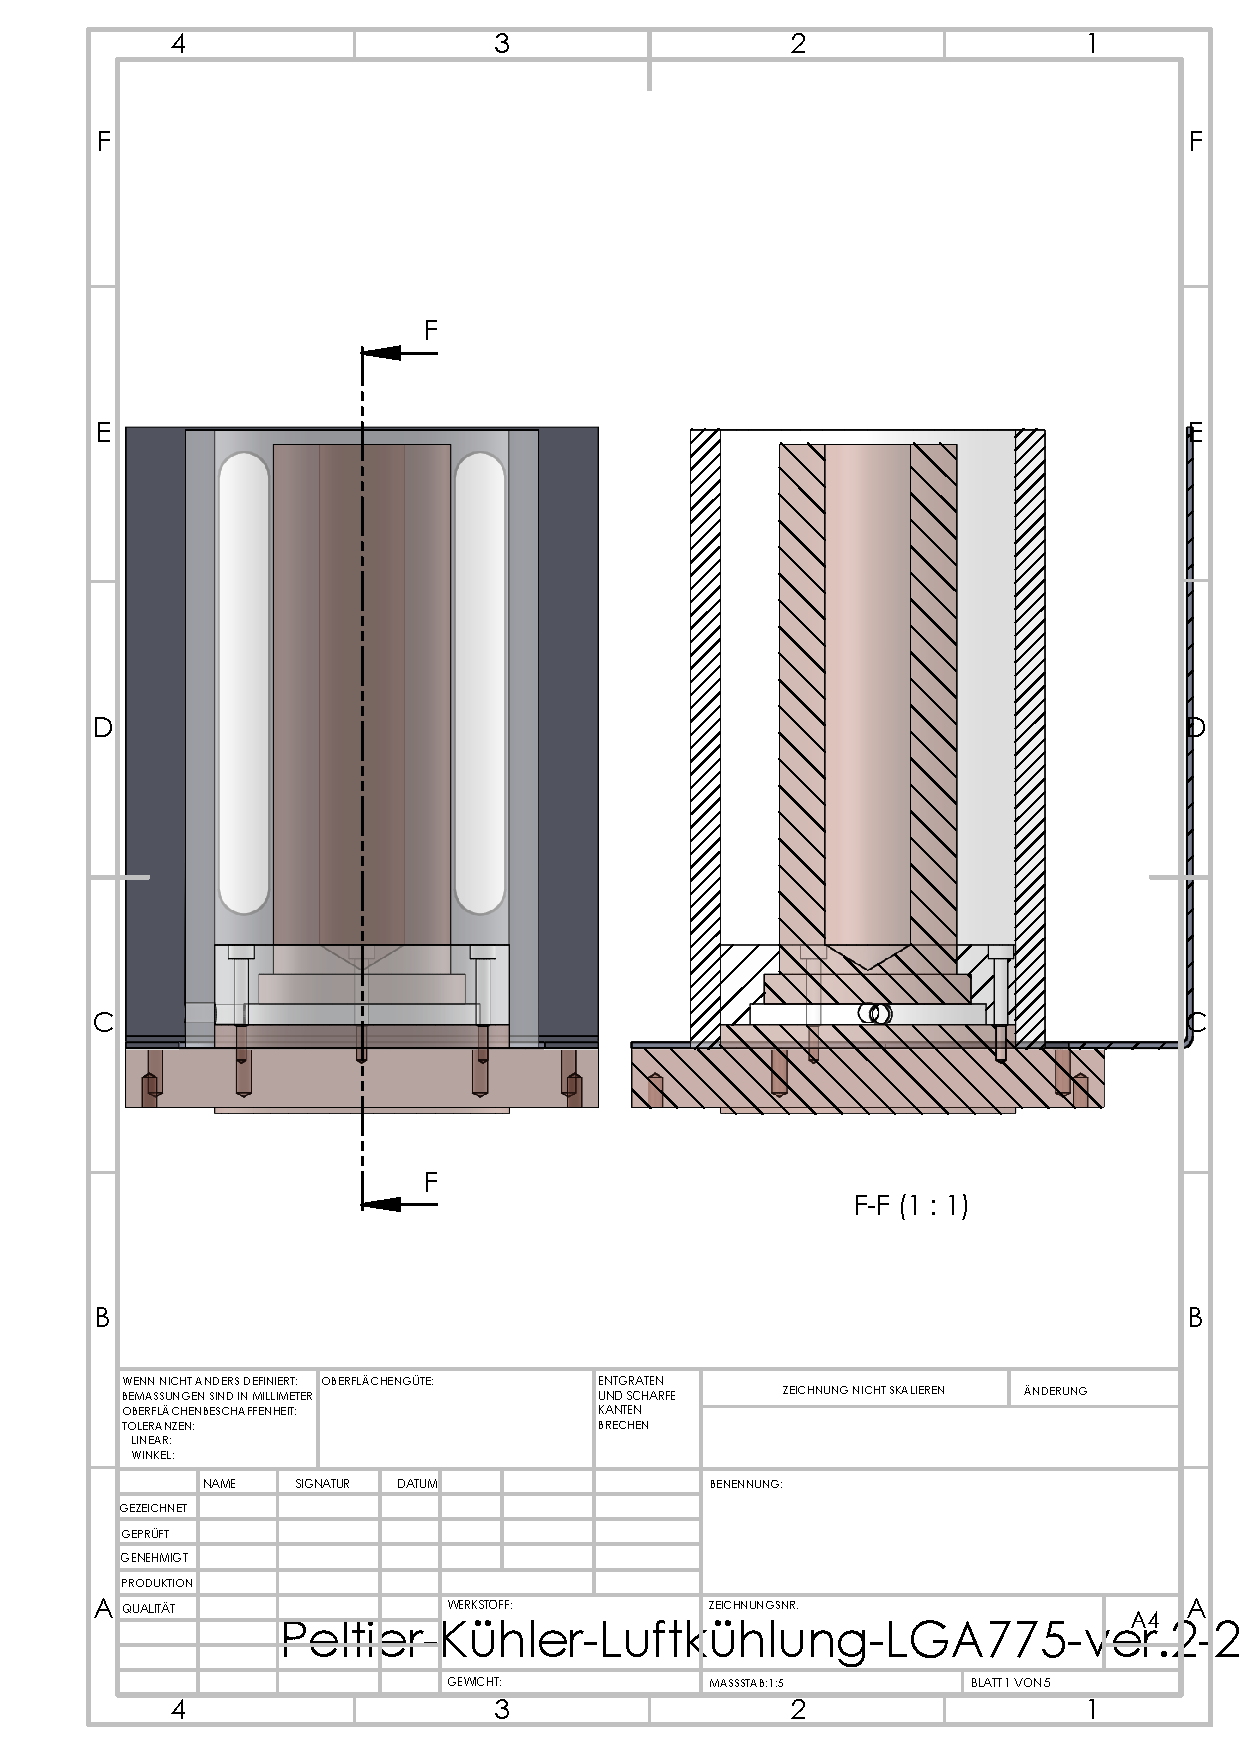
\includegraphics[width=0.7\textwidth]{./includes/chapter/backmatter/Peltier-LGA775.pdf}
\caption{Design of a peltier cooling unit used to store the liquid borazine precursor below \SI{5}{\celsius}. The precursor is surrounded by a rather tight fitting copper cylinder. Its thermal energy is permanently lowered by the peltier element that in turn rises the temperature of the lower copper plate. To keep it at room temperature, a CPU heat sink is attached (not shown in the sketch). A acrylic glass cylinder surrounds the cooled parts to prevent air moisture to condense and freeze on the copper. An "L" shaped mounting bracket with slotted holes ensures an easy fix of the cooler at the frame in various positions and angles.}
\label{fig:peltier-cooler}
\end{figure}
